\section{Basic Definitions}

\begin{definition}[Poset (partially ordered set)]
    A \textit{\textbf{poset}} $\mathbb{P}$ is a pair $\mathbb{P} = (X,P)$ where $X$ is a set and $P \subseteq X \times X$ is a relation that is
    \begin{itemize}
        \item reflexive: $\forall a \in X.\, (a,a) \in P$
        \item anti-symmetric: $a \neq b \land (a,b) \in P \implies (b,a) \not\in P$
        \item transitive: $(a,b) \in P \land (b,c) \in P \implies (a,c) \in P$
    \end{itemize}
\end{definition}

Instead of writing $(a,b) \in P$, we use the notation $a \leq_{\mathbb{P}} b$.

\begin{definition}[Embedding, Isomorphism, Automorphism]
    Given a poset $\mathbb{P} = (X,P)$ and $\mathbb{Q} = (Y,Q)$, an \textbf{embedding} from $\mathbb{P}$ into $\mathbb{Q}$ is an injective map $f:\; X \to Y$ with the property that $a \leq_{\mathbb{P}} b$ if and only if $f(a) \leq_{\mathbb{Q}} f(b)$. If the embedding is surjective, we call it an \textbf{isomorphism}. If $\mathbb{Q} = \mathbb{P}$, we call it an \textbf{automorphism}.
\end{definition}

For example, consider $X = \{\star, \circ, \diamond \}$ with $P = \{ (\star,\star), (\circ,\circ), (\diamond, \diamond), (\diamond, \star) \}$, and $Y = \{\star, \circ, \diamond, \Box \}$ with $Q = \{ (\star,\star), (\circ,\circ), (\diamond,\diamond), (\Box,\Box), (\Box,\star) \}$. Let $\mathbb{P} = (X,P)$ and $\mathbb{Q} = (Y,Q)$. Consider the function $f:\; X \to Y$ such that $f(\star) = \star$, $f(\circ) = \circ$, and $f(\diamond) = \Box$. $f$ is an embedding because $\diamond \leq_{\mathbb{P}} \star$ if and only if $f(\diamond) = \Box \leq_{\mathbb{Q}} \star = f(\star)$. However, $f$ is not an isomorphism because $\diamond$ is not in the range of $f$ so $f$ is not surjective.

\begin{definition}[Dual]
    Given a poset $\mathbb{P} = (X,P)$, we call the poset $\mathbb{P}^d = (X,P^d)$ where $a \leq_{\mathbb{P}^d} b \iff b \leq_{\mathbb{P}_d} a$ the \textbf{dual} of $\mathbb{P}$. We say a poset is self-dual if it is isomorphic to its dual.
\end{definition}

\begin{definition}[Cover]
    Given a poset $\mathbb{P} = (X,P)$ and a point $a \in X$, we say $a$ is \textbf{covered by} a point $b \in X$ if $a <_{\mathbb{P}} b$ and there is no $c$ such that $a <_{\mathbb{P}} c <_{\mathbb{P}} b$.
\end{definition}

\begin{definition}[Cover Graph]
    Given a poset $\mathbb{P} = (X,P)$, we call the graph $G = (X,E)$ given by $\{x,y\} \in E$ if and only if $x$ covers $y$ or $y$ covers $x$, the \textbf{cover graph} associated to $\mathbb{P}$. 
\end{definition}

If we draw the cover graph in an oriented fashion where lower vertices correspond to the $\leq_{\mathbb{P}}$-smaller elements, we have a special kind of cover graph known as \textbf{Hasse diagram}.

Let $\mathbb{P} = (X,P)$ be a poset where $X = \{a,b,c,d,e,f\}$ and $P = \{ (a,c), (b,c), (b,d), (d,e), (a,e), (e,f)\}$. One possible cover graph and the Hasse diagram is shown below.

\begin{figure}[htbp]
    \centering
    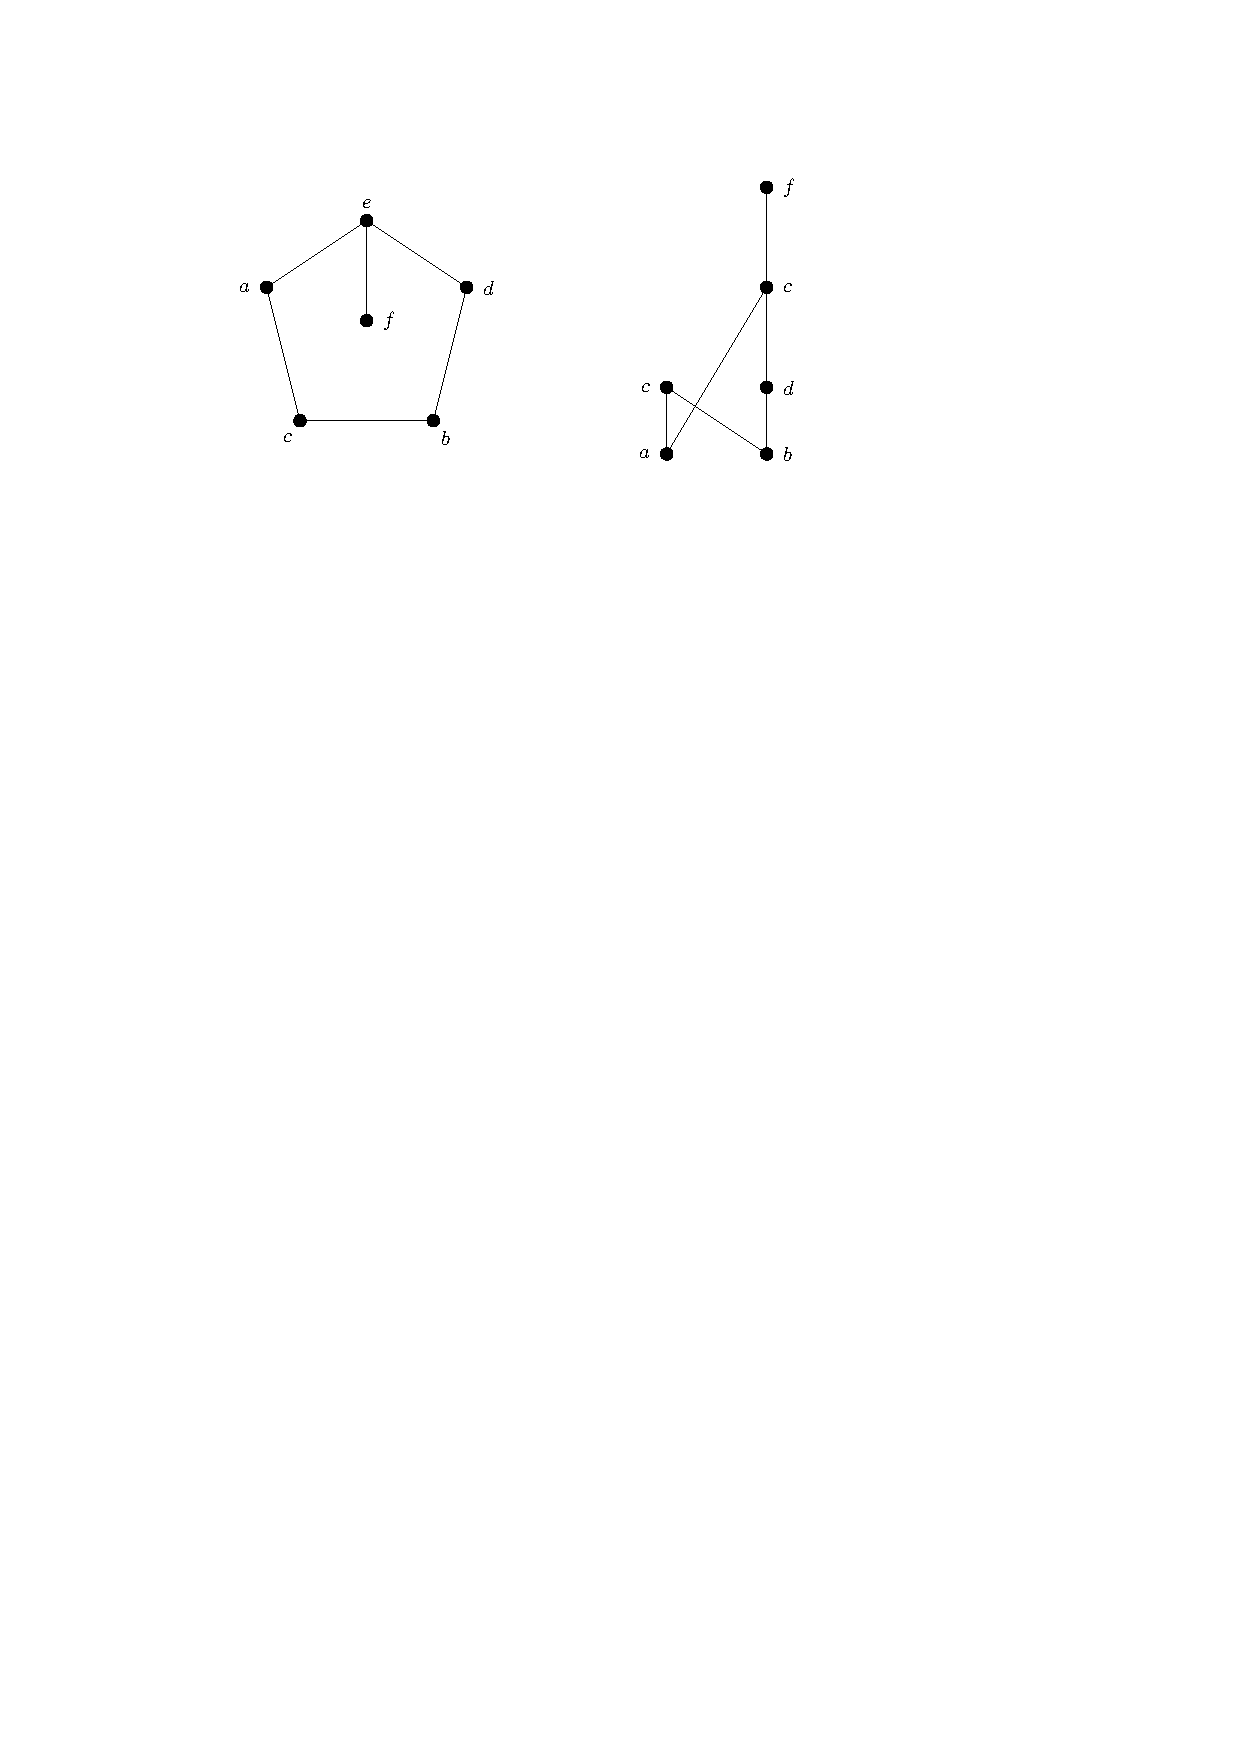
\includegraphics[width=0.5\linewidth]{figures/hasse-diagram.pdf}
    \caption{Cover graph and Hasse diagram for the poset described above.}
    \label{fig:hasse-diagram-example}
\end{figure}

\section{Linear Orders}

\begin{definition}[Comparability]
    Given a poset $\mathbb{P} = (X,P)$, we say two points $a,b \in X$ are \textit{\textbf{comparable}} if either $a <_{\mathbb{P}} b$ or $b <_{\mathbb{P}} b$ If two points are not comparable, we call them \textit{\textbf{incomparable}}.
\end{definition}

\begin{definition}[Total/Linear Order]
    Given a poset $\mathbb{P} = (X,P)$, we say $\mathbb{P}$ is \textit{\textbf{linearly ordered}} or \textit{\textbf{totally ordered}} if no two distinct points are incomparable.
\end{definition}

\section{Height and Width}

\begin{definition}[Antichain and Chain]
    Given a poset $\mathbb{P} = (X,P)$, we call $A \subseteq X$ an \textit{\textbf{antichain}} if every pair of distinct elements in $A$ are \textbf{incomparable}. We call a subset $C \subseteq X$ a \textit{\textbf{chain}} is every pair of distinct elements is \textbf{comparable}.
\end{definition}

\begin{definition}[Height and Width]
    Given a poset $\mathbb{P} = (X,P)$, we define the parameters $\mathsf{width}(\mathbb{P})$ and $\mathsf{height}(\mathbb{P})$ to denote the size of the largest antichain and chain of $\mathbb{P}$, respectively.
\end{definition}

\section{Subset Lattice and Sperner's Theorem}

\begin{theorem}[Sperner's Theorem]
    Consider the poset $\mathbb{P} = (\mathcal{P}([n]), \subseteq)$. Then, $\mathsf{width}(\mathbb{P}) = \binom{n}{\floor{n/2}}$.
\end{theorem}

\begin{proof}
    One can easily verify that $A = \{ S \subseteq [n] \mid |S| = \floor{\frac{n}{2}}\}$ is an \textbf{antichain}. Two sets of the same size are comparable if and only if they are equal. There are $\binom{n}{\floor{\frac{n}{2}}}$ such subsets of $[n]$ of size $\floor{\frac{n}{2}}$, so $\mathsf{width}(\mathbb{P}) \geq \binom{n}{\floor{\frac{n}{2}}}$. This shows that $\binom{n}{\floor{\frac{n}{2}}}$ is a lower bound.

    Now, we proceed to show that $\binom{n}{\floor{\frac{n}{2}}}$ is also an upper bound. Let $A = \{ S_1, \ldots, S_w \}$ be a \textbf{maximal antichain} of $\mathbb{P}$. It suffices to show that $w \leq \binom{n}{\floor{\frac{n}{2}}}$. For each $S_i \in A$, let $\mathcal{C}_i$ be the set of all \textbf{maximal chains} that contains $S_i$. We note that a maximal chain but be an $\subseteq$-increasing sequences that differs by at most one element per successive cover. If the next subset in the chain \textbf{differs} from the previous subset \textbf{by more than one element}, then the chain \textbf{would not be maximal}. In other words, starting from $S_i$, we remove 1 element until we reaches the empty set, and add 1 element until we reaches $[n]$. There are $|S_i|!$ ways to remove points successively from $S_i$. Similarly, there are $(k-|S_i|)!$ ways to add points successively to $S_i$. Therefore, for any $i$, $|\mathcal{C}_i| = |S_i|! \cdot (k-|S_i|)!$.

    \begin{figure}[htbp]
        \centering
        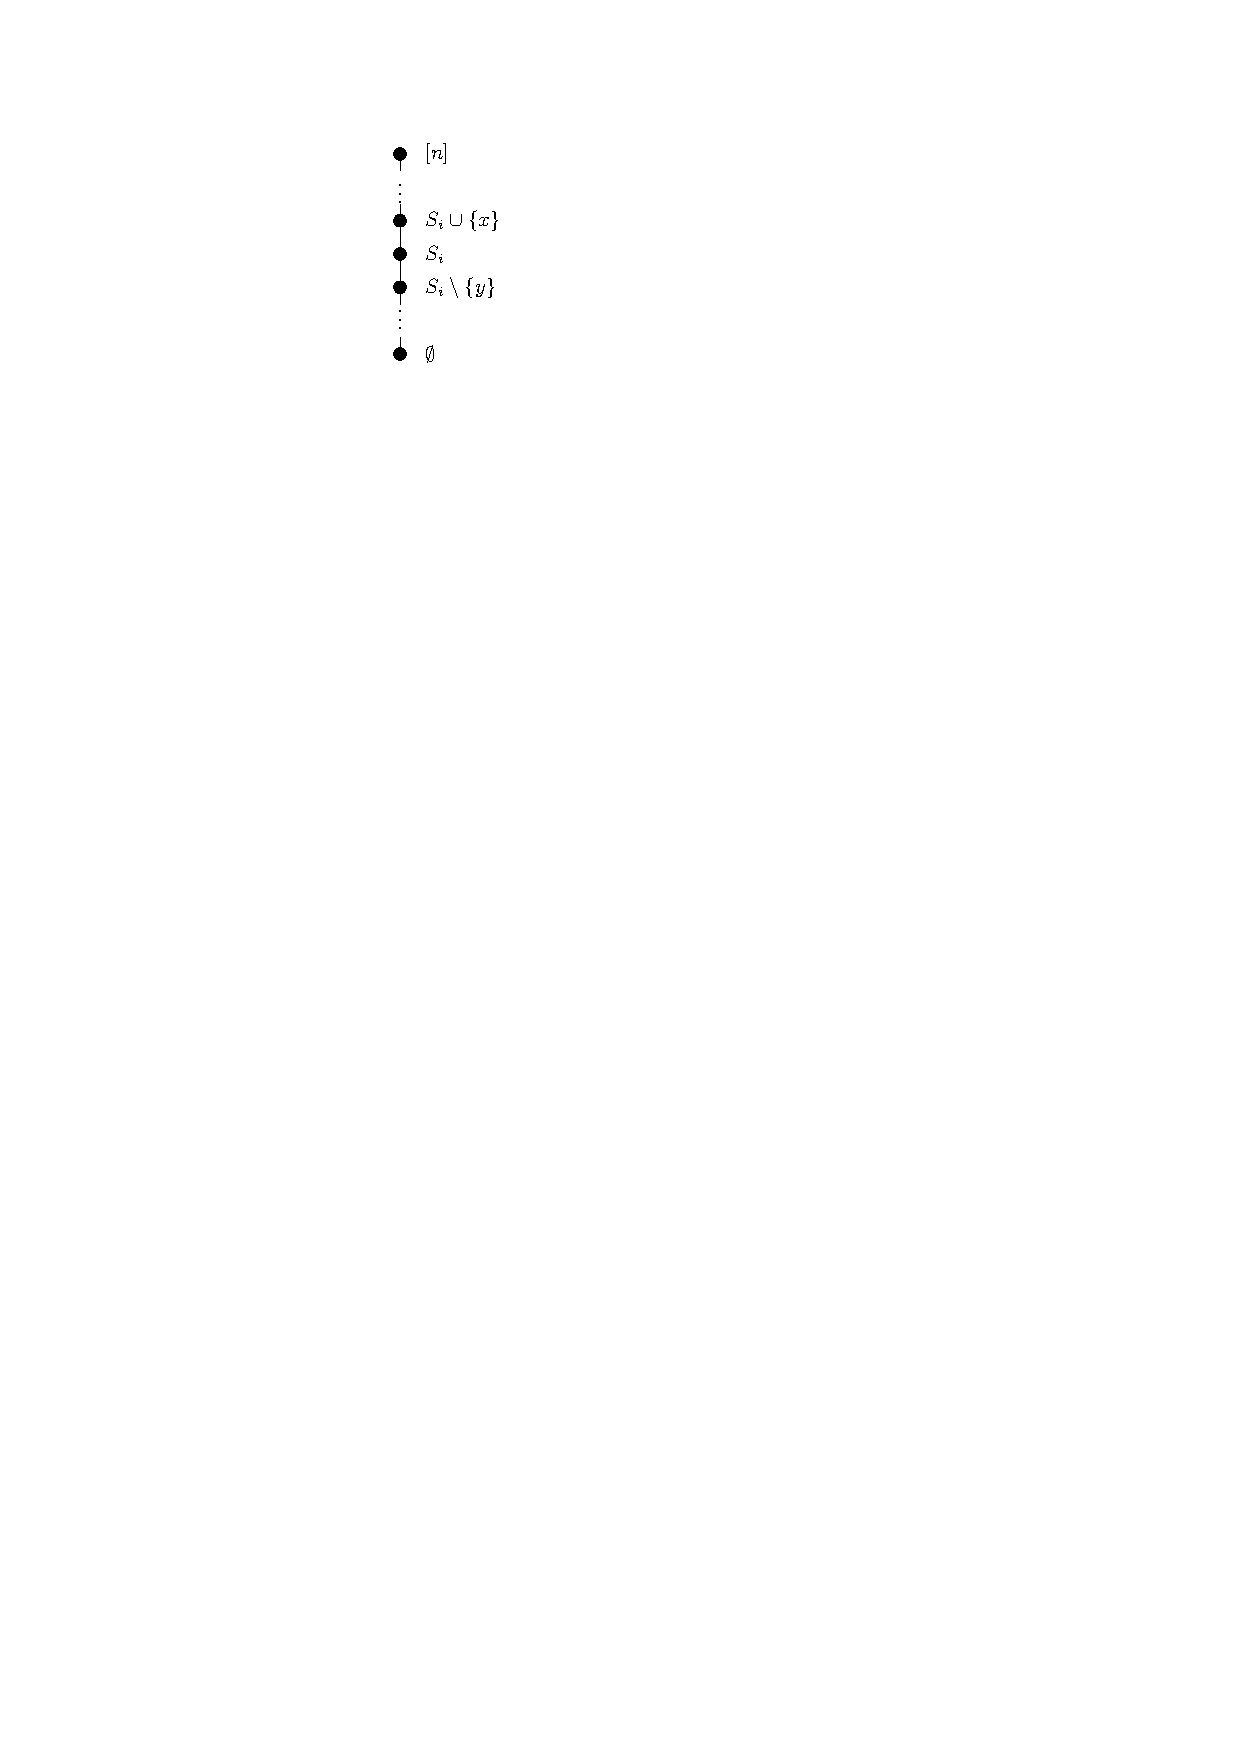
\includegraphics[width=0.1\linewidth]{figures/max-len-chain.pdf}
        \caption{Each subset must differ from the previous and next subset by exactly one element in a maximal chain. Otherwise, we form a chain of longer length by inserting a new subset in between.}
        \label{fig:max-len-chain}
    \end{figure}

    We also observe that there are exactly $n!$ many maximal chains, each corresponding to one ordering (permutation) to remove elements from $[n]$.

    For any $i \neq j$, $\mathcal{C}_i \cap \mathcal{C}_j = \emptyset$ because otherwise there would be a chain $C$ with $S_i,S_j \in C$ and hence $S_i$ and $S_j$ are comparable, which is a contradiction to our assumption that $S_i$ and $S_j$ are members of a maximal \textbf{antichain}. It follows that
    $$
    \left| \bigcup_{i=1}^w \mathcal{C}_i \right| = \sum_{i=1}^w |\mathcal{C}_i| \leq n!
    $$
    Since $|\mathcal{C}_i| = |S_i|! \cdot (k-|S_i|)!$, it follows that
    $$
    \sum_{i=1}^w |\mathcal{C}_i| = \sum_{i=1}^w (|S_i|! \cdot (k-|S_i|)!) \leq n!
    $$
    and hence
    $$
    \sum_{i=1}^w \frac{|S_i|! \cdot (k-|S_i|)!}{n!} = \sum_{i=1}^w \frac{1}{\binom{n}{|S_i|}} \leq 1
    $$
    by definition of combination. It follows from $\binom{n}{|S_i|} \leq \binom{n}{\floor{n/2}}$ that
    $$
    \sum_{i=1}^w \frac{1}{\binom{n}{\floor{n/2}}} \leq \sum_{i=1}^w \frac{1}{\binom{n}{|S_i|}}\leq 1
    $$
    and $w \leq \binom{n}{\floor{\frac{n}{2}}}$. Therefore, $\mathsf{width}(\mathbb{P}) \leq \binom{n}{\floor{\frac{n}{2}}}$ and because $\binom{n}{\floor{\frac{n}{2}}}$ is also a lower bound, $\mathsf{width}(\mathbb{P}) = \binom{n}{\floor{\frac{n}{2}}}$.
\end{proof}